\documentclass[]{auvsi_doc}
\setkeys{auvsi_doc.cls}{
	AUVSITitle={Airframe Subsystem Description},
	AUVSILogoPath={./../logo.pdf}
}

% include extra packages, if needed

\begin{document}

\begin{AUVSITitlePage}
\begin{artifacttable}
<<<<<<< HEAD
\entry{AF-008, 0.1, 02-19-19, Initial Draft for Subsystem Engineering, Tyler Critchfield, Ryan Anderson}
=======
\entry{AF-008, 0.1, 02-19-19, Initial Draft for SS Engineering, Tyler Critchfield, CHECKED BY}
>>>>>>> 252825537a102667548b948ee9ca0a781e8b2e28
% additional \entry{} commands for extra rows in the revision table, if needed
\end{artifacttable}
\end{AUVSITitlePage}

% document contents (see below for LaTex commands that make your life easier)
\section{Introduction}
This artifact describes the final design and modification of the Nimbus Pro airframe that was selected during the Concept Development stage. Images of the constructed airframe are included as well as a list of modifications we made to the plane. The advantages of the current concept in achieving our key success measures are described.

\section{Design Description}
The Nimbus Pro airframe is a fixed-wing plane with a large storage capacity and large wing span made of polystyrene (Fig. \ref{fig:plane1}). It was selected during Concept Development for its long span and spacious fuselage.

\begin{figure}[h!]
	\centering
	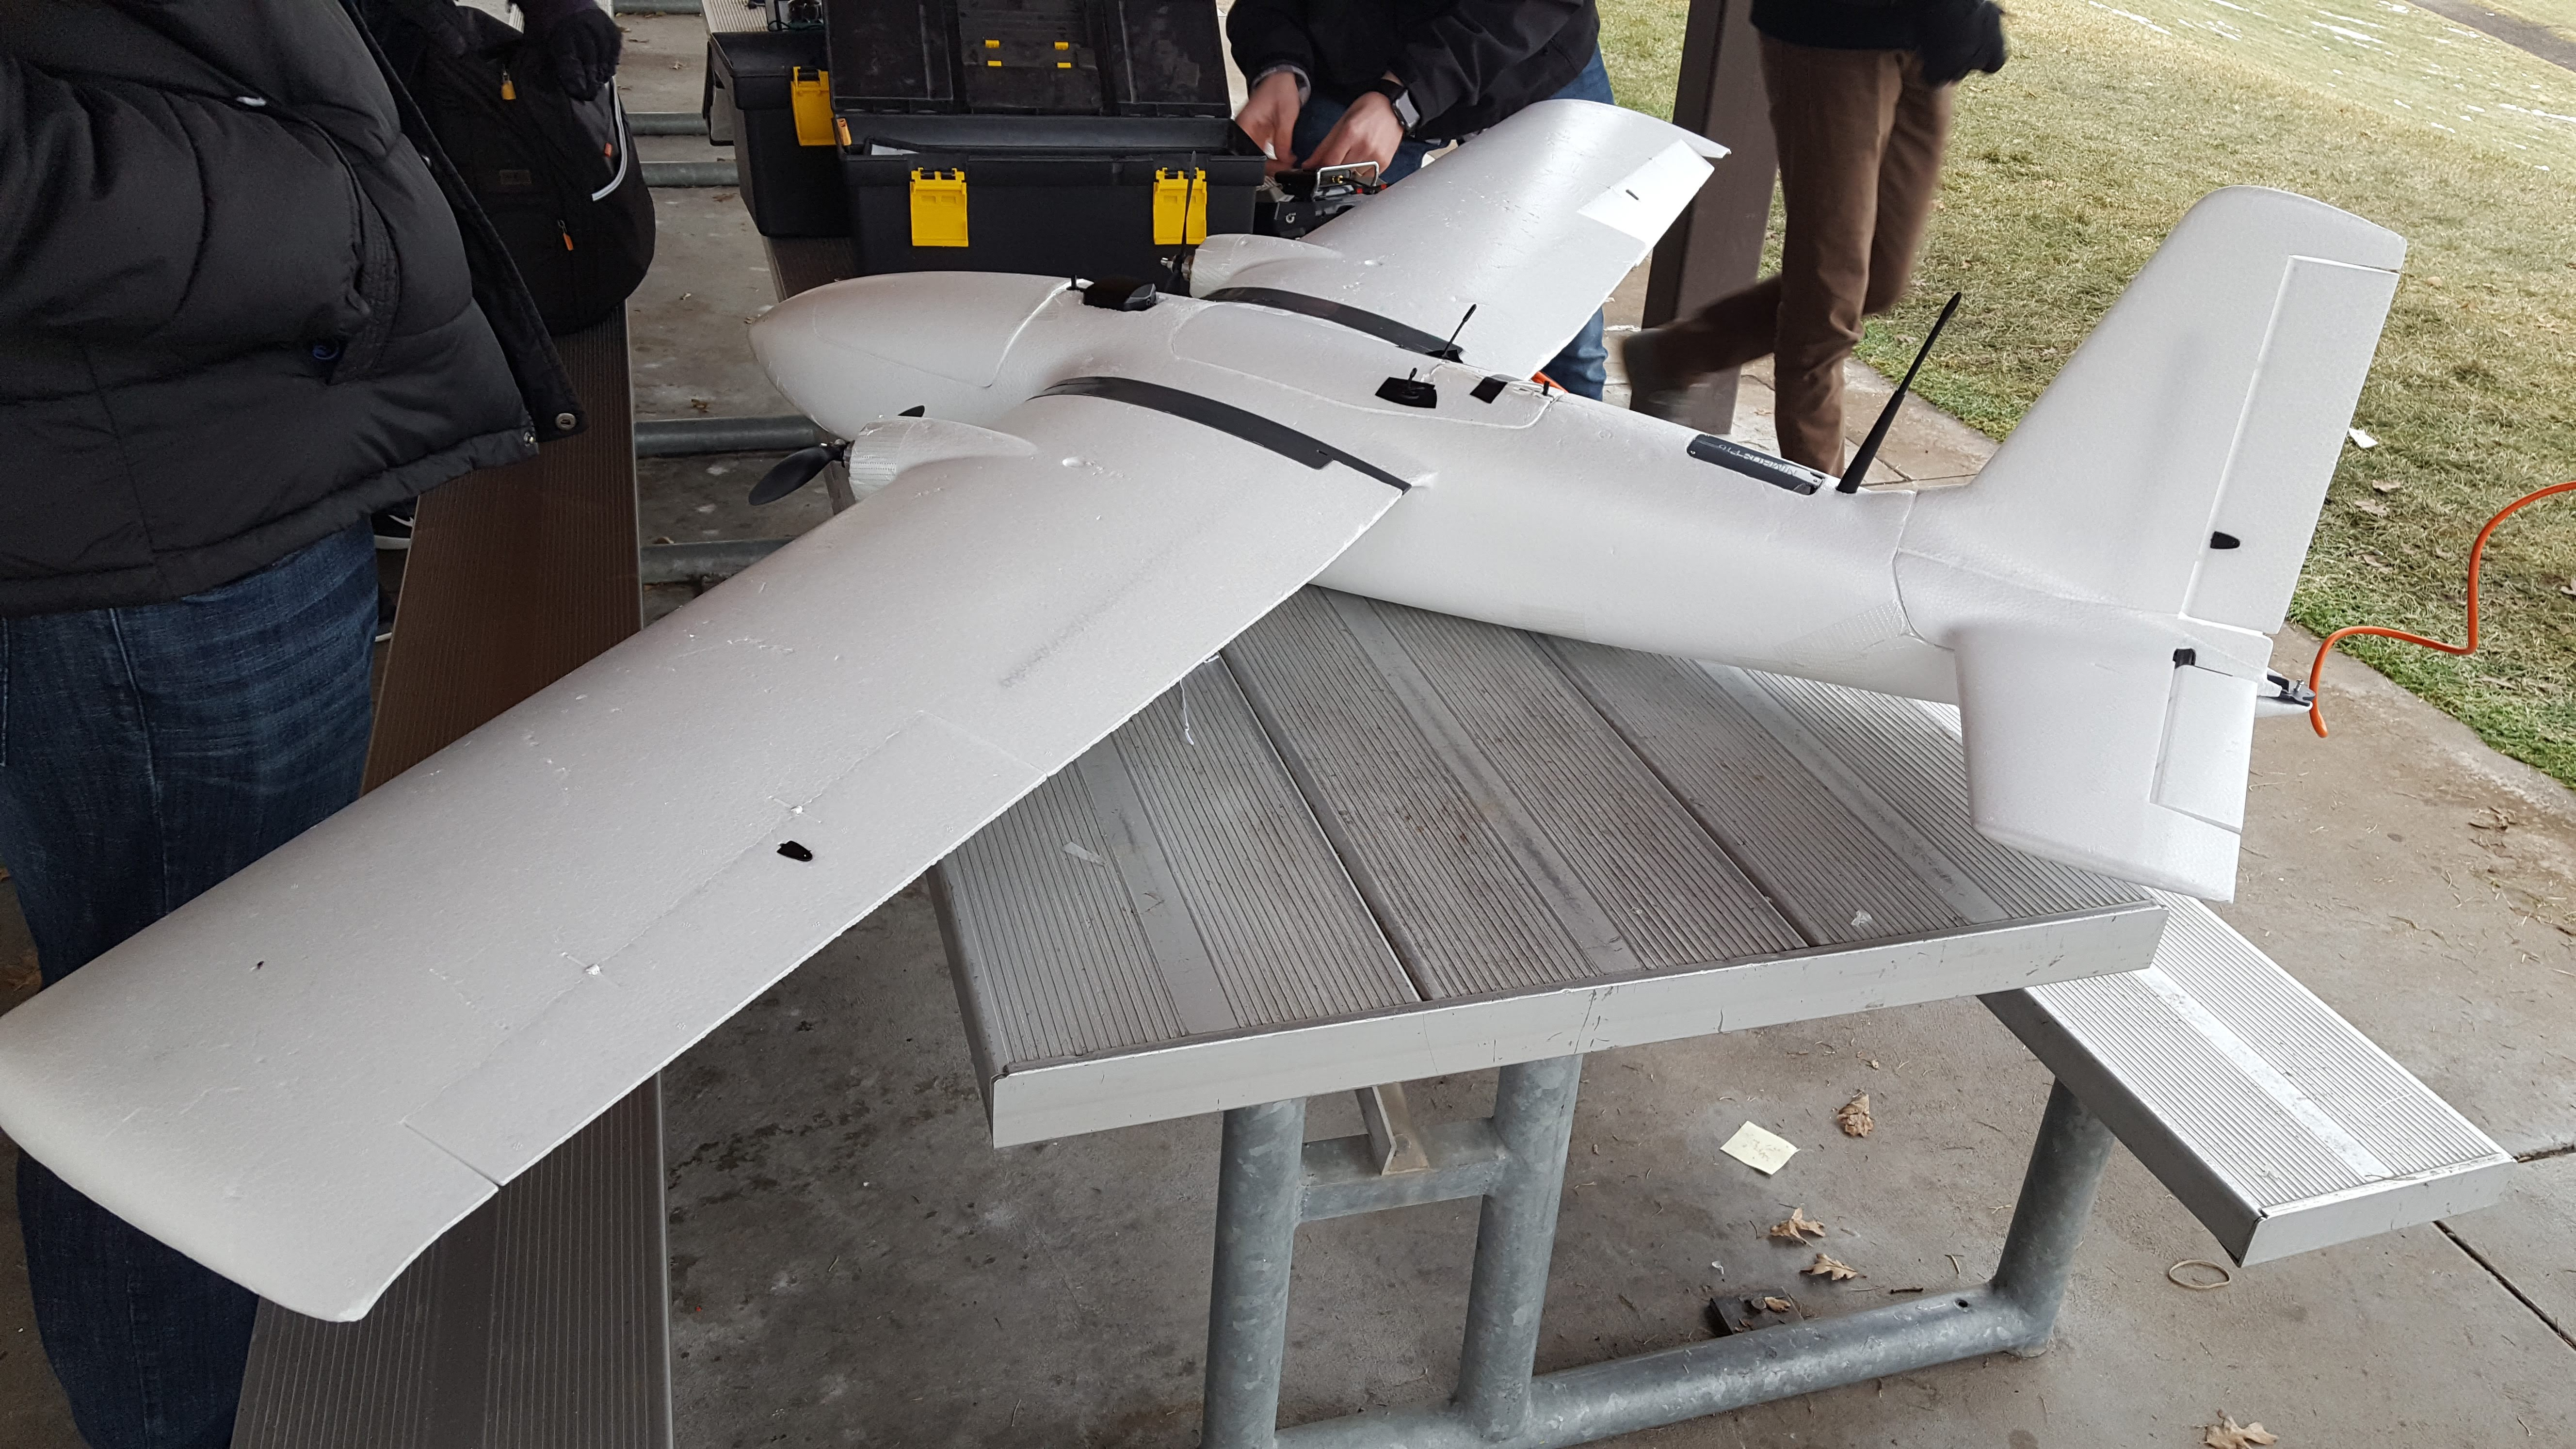
\includegraphics[width=.9\columnwidth]{figs/plane1}
	\caption{Fully-constructed Nimbus Pro airframe before its first flight.}
	\label{fig:plane1}
\end{figure} 

A detailed procedure for constructing the plane is beyond the scope of this artifact. It suffices to say that the procedure follows basic principles and steps of foam aircraft construction, as follows:

\begin{itemize}
	\item Glue fuselage sections together
	\item Attach proper servos and control horns to each control surface
	\item Attach motors and ESCs to wings
	\item Attach tail pieces
	\item Install all electronic hardware/wiring
	\item Ensure connectors and joints are properly secured and strengthened if necessary
	\item Attach/connect wings
\end{itemize}

The center of gravity (CG) was carefully placed to optimize performance using an aerodynamics model, as explained in AF-011. The following modifications were made to the airframe based on our application and integrated hardware:

\begin{itemize}
	\item Holes were made in the main compartment hatch for the R/C and Ubiquiti antennas. There is dedicated space further back in the plane for these components, but placing components there moved the CG back too far for an acceptable static margin. Care was also taken to space the Ubiquiti antenna far from the GPS antenna to avoid signal interference.
	\item The GPS slot on top was not used and taped over. The GPS was instead placed inside the nose of the plane to move the CG forward.
	\item The servos we selected were larger than the airframe was designed for. Because of this, some foam and plastic was removed from servo locations using razor blades, a hot metal tool, and wire cutters to allow them to fit.
	\item A foam wedge was inserted underneath the tail to increase the tail incidence angle (see further details below).
	\item Because the motor power wires are so thick, we bypassed the electrical connector that came with the airframe. Small holes were drilled into the wing connector pieces to allow for the large wires to extend from the ESCs in the wings to the fuselage. 
	\item In general, most components were placed as far forward as was reasonable to move our CG forward and increase our static margin. 
\end{itemize}

In Concept Development, we considered adding wing extensions to increase total span. This would help the plane fly slower by increasing lift. Flying at a lower velocity would then help us achieve higher performance in our key success measures (specifically obstacles hit, waypoint proximity, characteristics identified, and accuracy of payload drop). In order to decide if wing extensions would be worth, the aerodynamic benefits of extensions were modeled and compared to the relative cost of manufacture (See AF-012). In summary, it was decided that any extra benefit to extensions would not be worth the time and effort required to design, implement and test these extensions.

One unanticipated modification we've made to the aircraft is the placement of a foam wedge underneath the tail of the plane. Interestingly, the factory design has no tail incidence. Though we predicted problems, we decided to see if the plane would fly without this modification. It did fly, but it had a consistent tendency to want to pitch forward, making it difficult to take off and fly R/C. The plane was modeled and an incidence angle of $7.5^\circ$ determined the optimal condition (see AF-009 and AF-011). After installing the tail wedge, this problem was averted. The plane is now stable and flies very near the design speed we had originally planned for.

The tail wedge (see Fig. \ref{fig:wedge}) is made out of extruded polystyrene, measured and cut manually in order to give the required incidence angle for the tail. Several notches were carved into the top for it to securely fit with the tail connector pieces. Fiber tape was then wrapped around it to ensure it would not come loose during flight. The design drawing for the wedge is included in AF-010.

\begin{figure}[h!]
	\centering
	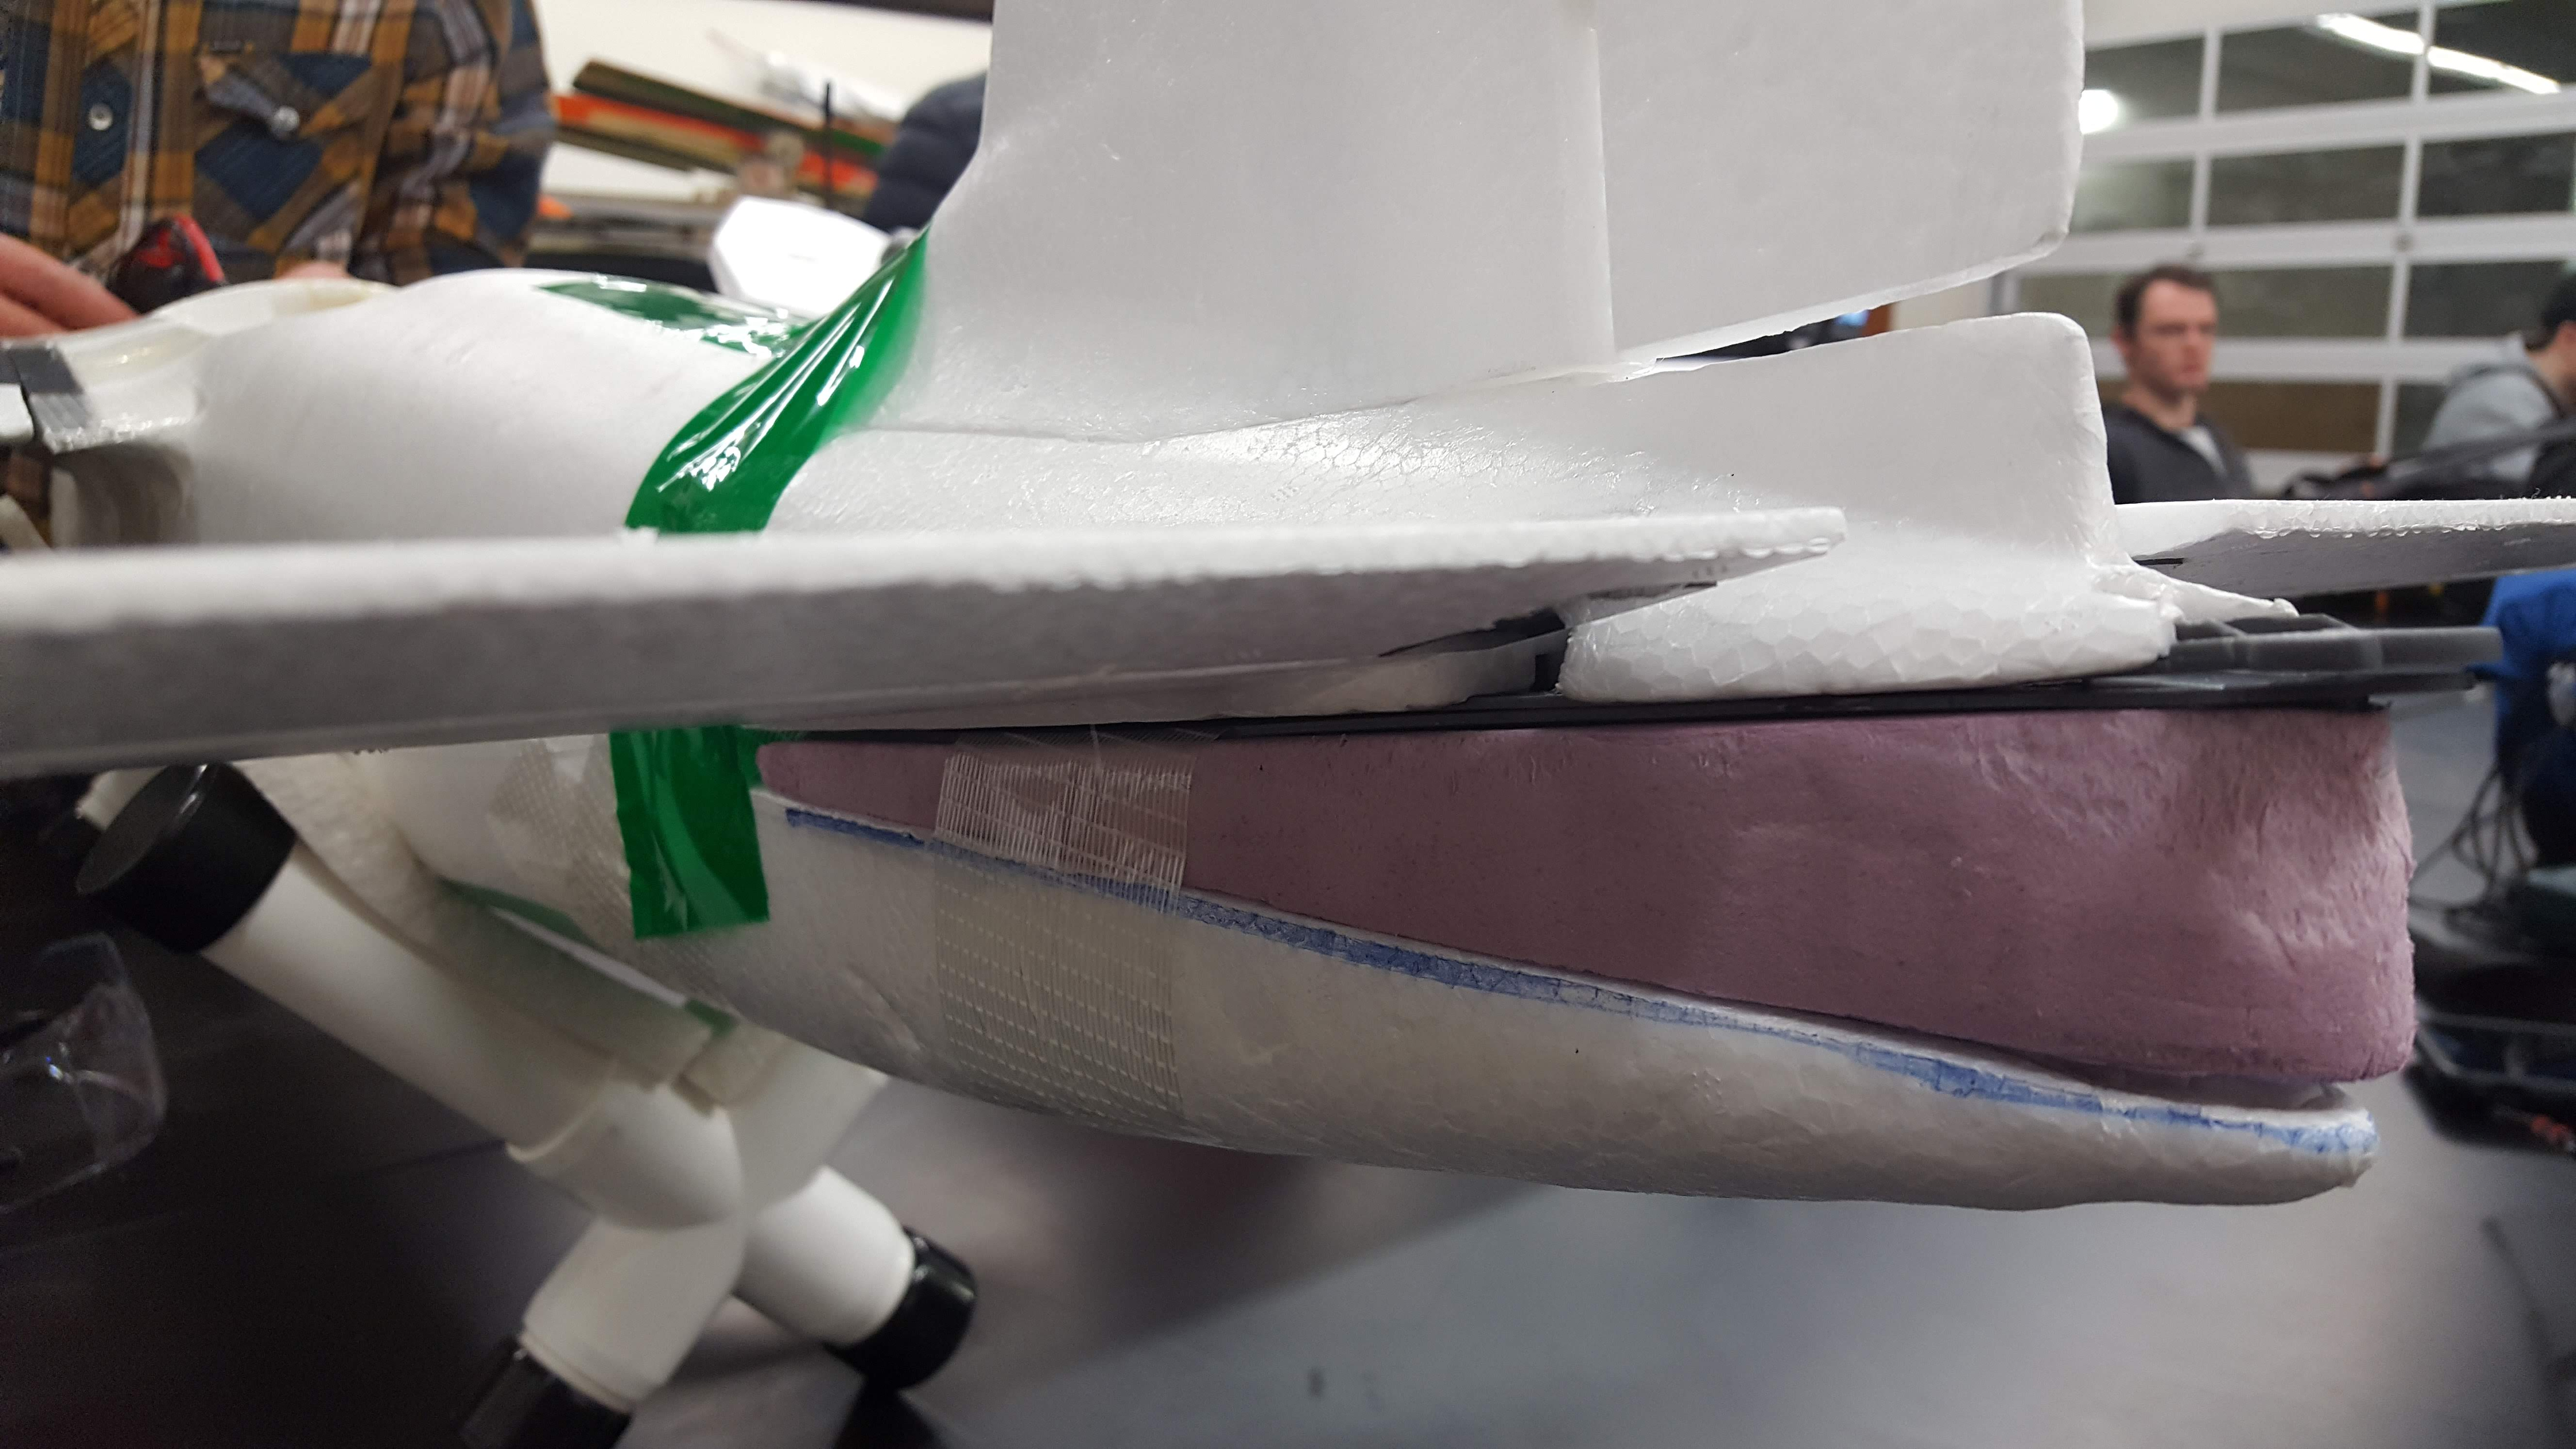
\includegraphics[width=.75\columnwidth]{figs/tailwedge}
	\caption{A foam tail wedge installed underneath the tail of the plane to increase its incidence angle and improve stability.}
	\label{fig:wedge}
\end{figure}

\section{Testing}
As described further in Artifact AF-013, we have done extensive flight testing to ensure our airframe performs as expected. In the past couple of months, we have had several successful flight tests with manual RC control and multiple successful flights while controlling with autopilot. While flying, it is very stable and flies at an average of ~15\ m/s. These outcomes show that our airframe works and is very capable to integrate with the other subsystems. Not only have we flown it with some autopilot control, we have also shown it can hold the imaging subsystem camera and the UGV subsystem. Both have demonstrated their subsystems can work with the plane while stationary, and we have yet to test them in flight. From these results, however, we are very confident our airframe will integrate well with these subsystems while in flight. 

\section{Conclusion}
Our airframe is fully assembled (with slight modifications) and has proven to consistently fly reliably. All of our key success measures depend on the airframe flying well - and many of them can be improved if the airframe flies with a low velocity. Our design and modifications ensure the airframe does fly slowly, which will help minimize obstacles hit, waypoint proximity, and error when dropping the UGV payload. It also improves image quality to identify more characteristics. The plane has flown successfully under R/C and autopilot control, the payload drop system has functioned successfully in flight, and the imaging subsystems have performed well inside the plane while stationary. We fully expect all three other subsystems to successfully integrate with the airframe during flight.

\end{document}
